\documentclass{report}
\usepackage[spanish]{babel}



\usepackage[spanish]{babel}
\usepackage[utf8x]{inputenc}
\usepackage{amsmath}
\usepackage{graphicx}
\usepackage[colorinlistoftodos]{todonotes}
\usepackage{enumitem}
\usepackage{listings}
\usepackage{verbatim}
\usepackage{eurosym}
\usepackage[export]{adjustbox}
\usepackage{amssymb}
\usepackage{bussproofs}
\usepackage{amsmath}
\usepackage{tikz}
\usepackage{xcolor}
\usepackage{listings}
\usepackage{titletoc}
\usepackage{hyperref}

\hypersetup{
  colorlinks=true,
  linkcolor=black,
  urlcolor=blue,
  citecolor=black
}

\newcommand{\coverPage}[6]{%
%----------------------------------------------------------------------------------------
%	COVER START
%----------------------------------------------------------------------------------------
\begin{titlepage}

    \newcommand{\HRule}{\rule{\linewidth}{0.5mm}}
    \newcommand{\department}{#1}
    \newcommand{\course}{#2}
    \newcommand{\titleValue}{#3}
    \newcommand{\subtitleValue}{#4}
    \newcommand{\authorName}{#5}

    \center

    %----------------------------------------------------------------------------------------
    %	HEADER
    %----------------------------------------------------------------------------------------
    
\includegraphics{images/logo_usa.png}
    \vspace{0.5cm}
    \textsc{\Large \department}\\[0.5cm]
    \textsc{\Large \course}\\[0.5cm]
    \vfill

    %----------------------------------------------------------------------------------------
    %	TITLE
    %----------------------------------------------------------------------------------------

    \HRule\\
    \Huge
    \textbf{\titleValue}\\[0.5cm]
    \Large
    \textbf{\subtitleValue}\\
    \HRule\\[0.5cm]

    %----------------------------------------------------------------------------------------
    %	AUTHOR AND DATE
    %----------------------------------------------------------------------------------------

    \vfill
    \Large
    \textit{\authorName}\\
    {\large \today}\\[2cm]

\end{titlepage}
%----------------------------------------------------------------------------------------
%	COVER END
%----------------------------------------------------------------------------------------
}

\begin{document}
    \coverPage{ Matemáticas }{ Álgebra Lineal II }{ Tarea 4 }{  }{ Alexander Mendoza }{\today}

    \section*{Tarea}
    \begin{enumerate}
        \item Mostrar que el conjunto $B=\{1,x,2x^2-1\}$ esta en $p^2[-1,1]$ al producto punto $<f.g>=\int_0^1\frac{f(x)g(x)}{\sqrt{1-x^2}}$, si es ortonogonal, entonces obtenga la base ortonormal.
    
        Para verificar si es ortogonal, tenemos que ver que:
    
        \begin{itemize}
            \item     Sea $f(x)=1$ y $g(x)=x$, tenemos lo siguiente:
            $$<f,g>=\int_{-1}^1\frac{1x}{\sqrt{1-x^2}}dx$$ Como la función es impar y esta en un intervalo simétrico, podemos asegurar que la integral es cero.
            \item  Sea $f(x)=x$ y $g(x)=2x^2-1$, tenemos lo siguiente:
    
            $$<f,g>=\int_{-1}^1\frac{x(2x^2-1)}{\sqrt{1-x^2}}dx$$
    
            Como la función es impar y esta en un intervalo simétrico, podemos asegurar que la integral es cero.
            \item     Sea $f(x)=1$ y $g(x)=x$, tenemos lo siguiente:
            $$<f,g>=\int_{-1}^1\frac{2x^2-1}{\sqrt{1-x^2}}dx=\int_{-1}^1\frac{2x^2}{1-x^2}-\int_{-1}^1\frac{1}{\sqrt{1-x^2}}=\pi-\pi=0$$ Como la función es impar y esta en un intervalo simétrico, podemos asegurar que la integral es cero.
    
        \end{itemize}
           
    
        Como ya comprobamos que es ortogonal, obtengamos la base:
    
        \begin{itemize}
            \item Paso 1: $$h_1(x)=\frac{1}{||1||}=1$$
            \item Paso 2: $$g_2(x)=x-<x,1>1=x-\int_{-1}^1\frac{x}{\sqrt{1-x^2}}=x$$ $$h_2(x)=\frac{g_2(x)}{||g_2(x)||}=\frac{x}{\int_{-1}^1\frac{x^2}{\sqrt{1-x^2}}dx}=\frac{x}{\sqrt{\frac{\pi}{2}}}=\frac{x\sqrt{2\pi}}{\pi}$$
            \item Paso 3: $$g_3(x)=2x^2-1-<2x^2-1,x>x-<2x^2,\frac{x\sqrt{2\pi}}{\pi}>\frac{x\sqrt{2\pi}}{\pi}$$
            
            \begin{align*}
            &= 2x^2 - 1 - \int_{-1}^1 \frac{2x^2 - 1}{\sqrt{1-x^2}} \, dx - \left(\int_{-1}^1 \frac{(x^2 - 1)\left(\frac{x\sqrt{2\pi}}{\pi}\right)}{\sqrt{1-x^2}} \, dx\right)\left( \frac{x\sqrt{2\pi}}{\pi}\right)
            \end{align*}
            \begin{align*}
            &= 2x^2-1-0-\left(\frac{\sqrt{2\pi}}{\pi}\int_{-1}^1\frac{(2x^2-1)x}{\sqrt{1-x^2}}\right)\left(\frac{x\sqrt{2\pi}}{\pi}\right)=2x^2-1
            \end{align*}
        \end{itemize}
    
      De esta manera tenemos que: $C=\{1,\frac{x\sqrt{2\pi}}{\pi},2x^2-1\}$
    \begin{figure}[h]
    \centering
    

    \begin{center}
    \fbox{\adjustbox{trim=1 1 1 1, height=3cm}{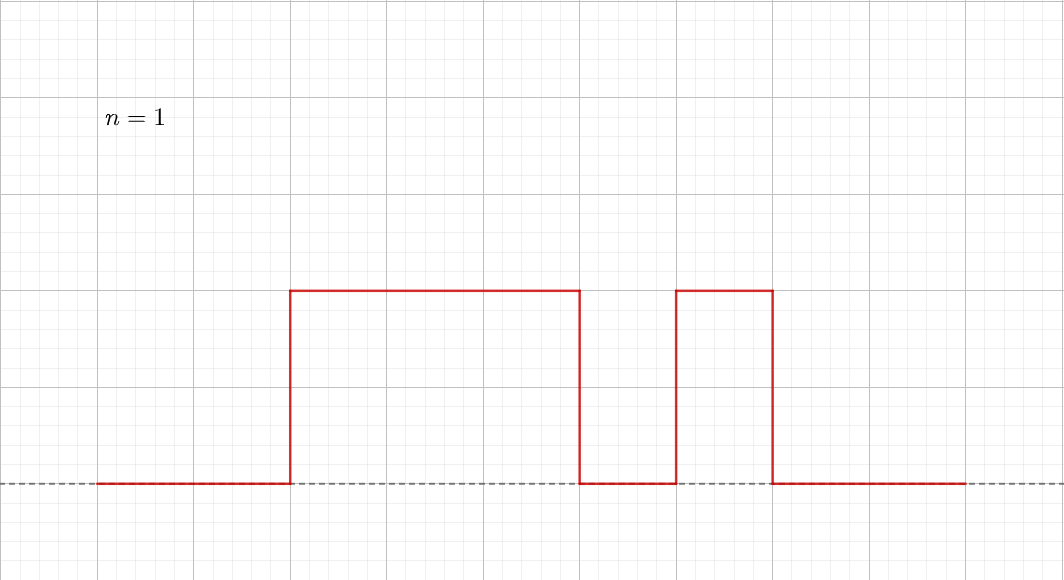
\includegraphics{images/1.png}}}
    \end{center}
    
    
    \end{figure}
        \item $||A||_F=\sqrt{tr(A^*A)}$\\
    
        Matrices pauli: $$B=\left\{
      \frac{1}{\sqrt{2}}\begin{pmatrix}
    1 & 0\\
    0 & 1
    \end{pmatrix}, \quad
    \frac{1}{\sqrt{2}}\begin{pmatrix}
    0 & 1 \\
    1 & 0
    \end{pmatrix}, \quad
    \frac{1}{\sqrt{2}} \begin{pmatrix}
    0 & -i \\
    i & 0
    \end{pmatrix}, \quad
    \frac{1}{\sqrt{2}} \begin{pmatrix}
    1 & 0 \\
    0 & -1
    \end{pmatrix}\right\}
    $$    
    \\$V=M_{2x2}(C)$, con producto frobenius
    
    
    
    \begin{enumerate}[label=\alph*)]
        \item Mostrar que $B$ es una base ortonormal para V
                \begin{enumerate}
                    \item  $\sqrt{tr(M_1)(M_2^*)}=\sqrt{tr\begin{pmatrix}
    \frac{1}{\sqrt{2}}\ & 0\\
    0 & \frac{1}{\sqrt{2}}\
    \end{pmatrix} \cdot \begin{pmatrix}
    0 & \frac{1}{\sqrt{2}}\\
    \frac{1}{\sqrt{2}} & 0\\
    \end{pmatrix}}=\sqrt{tr\begin{pmatrix}
    0 & \frac{1}{\sqrt{2}}\\
    \frac{1}{\sqrt{2}} & 0\\
    \end{pmatrix}}=\sqrt{0}=0 $
    
    
    
    
     
    \item $\sqrt{\text{tr}(M_1 M_3^*)} = \sqrt{\text{tr} \begin{pmatrix}
    \frac{1}{\sqrt{2}} & 0\\
    0 & \frac{1}{\sqrt{2}}
    \end{pmatrix} \cdot \frac{1}{\sqrt{2}}\begin{pmatrix}
    0 & \frac{-i}{\sqrt{2}}\\
    \frac{i}{\sqrt{2}} & 0
    \end{pmatrix}  }= \sqrt{\text{tr}  \begin{pmatrix}
    0 & \frac{-i}{\sqrt{2}}\\
    \frac{i}{\sqrt{2}} & 0
    \end{pmatrix} } = \sqrt{0} = 0 $
    
    
    
    
    
    
    
    
    \item $\sqrt{\text{tr}(M_1 M_4^*)} = \sqrt{\text{tr}  \begin{pmatrix}
    \frac{1}{\sqrt{2}} & 0\\
    0 & \frac{1}{\sqrt{2}}
    \end{pmatrix} \cdot \frac{1}{\sqrt{2}}\begin{pmatrix}
    \frac{1}{\sqrt{2}} & 0\\
    0 & \frac{-1}{\sqrt{2}}
    \end{pmatrix}}= \sqrt{\text{tr}   \begin{pmatrix}
    \frac{1}{\sqrt{2}} & 0\\
    0 & \frac{-1}{\sqrt{2}}
    \end{pmatrix}} = \sqrt{0} = 0 $
    
    
     
    
     
    \item $\sqrt{\text{tr}(M_2 M_3^*)} = \sqrt{\text{tr} \begin{pmatrix}
    0 & \frac{1}{\sqrt{2}}\\
    \frac{1}{\sqrt{2}} & 0
    \end{pmatrix} \cdot \begin{pmatrix}
    0 & \frac{i}{\sqrt{2}}\\
    \frac{-i}{\sqrt{2}} & 0
    \end{pmatrix}  }= \sqrt{\text{tr}  \begin{pmatrix}
    \frac{-i}{\sqrt{2}} & 0\\
    0 & \frac{i}{\sqrt{2}}
    \end{pmatrix}} = \sqrt{0} = 0 $
    
    
    
    \item $\sqrt{\text{tr}(M_2 M_4^*)} = \sqrt{\text{tr} \begin{pmatrix}
    0 & \frac{1}{\sqrt{2}}\\
    \frac{1}{\sqrt{2}} & 0
    \end{pmatrix} \cdot \frac{1}{\sqrt{2}}\begin{pmatrix}
    \frac{1}{\sqrt{2}} & 0\\
    0 & \frac{-1}{\sqrt{2}}
    \end{pmatrix}  }= \sqrt{\text{tr}  \begin{pmatrix}
    0 & \frac{-1}{\sqrt{2}}\\
    \frac{1}{\sqrt{2}} & 0
    \end{pmatrix} } = \sqrt{0} = 0 $
    
    
     
    \item  $\sqrt{\text{tr}(M_3 M_4^*)} = \sqrt{\text{tr} \begin{pmatrix}
    0 & \frac{-i}{\sqrt{2}}\\
    \frac{i}{\sqrt{2}} & 0
    \end{pmatrix} \cdot \frac{1}{\sqrt{2}}\begin{pmatrix}
    \frac{1}{\sqrt{2}} & 0\\
    0 & \frac{-1}{\sqrt{2}}
    \end{pmatrix}  }= \sqrt{\text{tr} \frac{1}{2} \begin{pmatrix}
    0 & \frac{i}{\sqrt{2}}\\
    \frac{i}{\sqrt{2}} & 0
    \end{pmatrix} } = \sqrt{0} = 0 $
    
    
    Ahora miramos que al hacer el producto de frobenius de las matrices con ellas mismas debe dar 1:
    
    
    
     
    \item $ \sqrt{\text{tr}(M_1 M_1^*)} =\sqrt{\text{tr} \begin{pmatrix}
    \frac{1}{\sqrt{2}}& 0\\
    0 & \frac{1}{\sqrt{2}}
    \end{pmatrix} \cdot \begin{pmatrix}
    \frac{1}{\sqrt{2}} & 0\\
    0 & \frac{1}{\sqrt{2}}
    \end{pmatrix}}= \sqrt{\text{tr} \begin{pmatrix}
    \frac{1}{2} & 0 \\
    0 & \frac{1}{2}
    \end{pmatrix}} = \sqrt{1} = 1$
    
    
    \item $ \sqrt{\text{tr}(M_2 M_2^*)} =\sqrt{\text{tr} \begin{pmatrix}
    0& \frac{1}{\sqrt{2}}\\
    \frac{1}{\sqrt{2}} & 0
    \end{pmatrix} \cdot \begin{pmatrix}
    0& \frac{1}{\sqrt{2}}\\
    \frac{1}{\sqrt{2}} & 0
    \end{pmatrix}}= \sqrt{\text{tr} \begin{pmatrix}
    \frac{1}{2} & 0 \\
    0 & \frac{1}{2}
    \end{pmatrix}} = \sqrt{1} = 1$ 
    
    
    \item $ \sqrt{\text{tr}(M_3 M_3^*)} =\sqrt{\text{tr} \begin{pmatrix}
    0& \frac{-i}{\sqrt{2}}\\
    \frac{i}{\sqrt{2}} & 0
    \end{pmatrix} \cdot \begin{pmatrix}
    0& \frac{-i}{\sqrt{2}}\\
    \frac{i}{\sqrt{2}} & 0
    \end{pmatrix}}= \sqrt{\text{tr} \begin{pmatrix}
    \frac{1}{2} & 0 \\
    0 & \frac{1}{2}
    \end{pmatrix}} = \sqrt{1} = 1$ 
    
    \item $ \sqrt{\text{tr}(M_1 M_1^*)} =\sqrt{\text{tr} \begin{pmatrix}
    \frac{1}{\sqrt{2}}& 0\\
    0 & \frac{-1}{\sqrt{2}}
    \end{pmatrix} \cdot \begin{pmatrix}
    \frac{1}{\sqrt{2}} & 0\\
    0 & \frac{-1}{\sqrt{2}}
    \end{pmatrix}}= \sqrt{\text{tr} \begin{pmatrix}
    \frac{1}{2} & 0 \\
    0 & \frac{1}{2}
    \end{pmatrix}} = \sqrt{1} = 1$
    
    Así hemos demostrado que la base es linealmente independiente.
    
    \end{enumerate}
    
    \newpage
    \item $[A]_B$ donde A$=\begin{pmatrix}
        5 &2-3i\\
        2+3i & -3
    \end{pmatrix}$.
    \begin{itemize}
        \item $\begin{pmatrix}
        5 &2-3i\\
        2+3i & -3
    \end{pmatrix}\cdot\begin{pmatrix}
        \frac{1}{\sqrt{2}}& 0 \\
        0 & \frac{1}{\sqrt{2}}
    \end{pmatrix}= \left( 5\cdot\frac{1}{\sqrt{2}}\right) + 0 \left(2-3i\right) + 0\left(2+3i\right) - 3\left(\frac{1}{\sqrt{2}}\right)
    \\=\frac{5}{\sqrt{2}}-\frac{3}{\sqrt{2}}=\frac{2}{\sqrt{2}}=c_1$
    
    \item $\begin{pmatrix}
        5 &2-3i\\
        2+3i & -3
    \end{pmatrix}\cdot\begin{pmatrix}
       0& \frac{1}{\sqrt{2}} \\
        \frac{1}{\sqrt{2}} & 0
    \end{pmatrix}= \frac{2-3i}{\sqrt{2}}+\frac{2+3i}{\sqrt{2}}=2\sqrt{2}=c_2$
    
    \item $\begin{pmatrix}
        5 &2-3i\\
        2+3i & -3
    \end{pmatrix}\cdot\begin{pmatrix}
       0& \frac{-i}{\sqrt{2}} \\
        \frac{i}{\sqrt{2}} & 0
    \end{pmatrix}=\frac{(2-3i)(-i)}{\sqrt{2}}+\frac{(2+3i)(-i)}{\sqrt{2}}=\frac{2i+3i^2+2i+3i^2}{\sqrt{2}}=\frac{3(-1+3(-1))}{\sqrt{2}}=\frac{6}{\sqrt{2}}=c_3$
    
    \item \item $\begin{pmatrix}
        5 &2-3i\\
        2+3i & -3
    \end{pmatrix}\cdot\begin{pmatrix}
        \frac{1}{\sqrt{2}}& 0 \\
        0 & \frac{1}{\sqrt{2}}
    \end{pmatrix}= \frac{5}{\sqrt{2}}+\frac{3}{\sqrt{2}}=\frac{8}{\sqrt{2}}=c_4$
    \end{itemize}
    
    Vamos a verificar, multiplicando $C_1,c_2,c_3,c_4$ con las matrices y luego sumarlas, deberia darnos la matriz A:
    
    $=\frac{2}{\sqrt{2}}\left[\begin{array}{cc}
    \frac{1}{\sqrt{2}} & 0 \\
    0 & \frac{1}{\sqrt{2}}
    \end{array}\right]+2 \sqrt{2}\left[\begin{array}{cc}
    0 & \frac{1}{\sqrt{2}} \\
    \frac{1}{\sqrt{2}} & 0
    \end{array}\right]+\frac{6}{\sqrt{2}}\left[\begin{array}{cc}
    0 & \frac{-i}{\sqrt{2}} \\
    \frac{i}{\sqrt{2}} & 0
    \end{array}\right]+\frac{8}{\sqrt{2}}\left[\begin{array}{cc}
    \frac{1}{\sqrt{2}} & 0 \\
    0 & \frac{-1}{\sqrt{2}}
    \end{array}\right]=$\\
    $=\begin{pmatrix}
        1 &0\\
        0 & 1
    \end{pmatrix}+\begin{pmatrix}
        0 &2 \\
        2 & 0
    \end{pmatrix}+\begin{pmatrix}
        0 & -3i\\
        3i & 0
    \end{pmatrix}+\begin{pmatrix}
        4 & 0\\
        0 & -4
    \end{pmatrix}=\left[\begin{matrix}5 & 2 - 3 i\\3 i + 2 & -3\end{matrix}\right]$
    
    
    Por tanto tenemos que: $$[A]_B=\{c_1,c_2,c_3,c_4\}=\frac{2}{\sqrt{2}}.2\sqrt{2},\frac{6}{\sqrt{2}},\frac{8}{\sqrt{2}}$$
    \end{enumerate}
    \end{enumerate}
    
    \newpage 
    \section*{Ejercicios aula virtual}
    
    \begin{enumerate}
        \item a) Si Q es  ortogonal, como usted sabe que Q es invertible y $Q^{-1}$ también es ortogonal. \\
        b)Si $Q_1^{T}=Q_1^{-1}$ y $Q_2^{T}=Q_2^{-1}$ demuestre que $Q_1,Q-2$ también es una matriz ortogonal.
        \\
        a) \begin{align*}
        &I = I  \\
        &Q^{-1}  = Q^{-1} & &\text{(Propiedad reflexiva)} \\
        &Q^{-1}  = Q^\top & &\text{(Definición de matriz ortogonal)} \\
        &(Q^{-1})^\top  = (Q^\top)^\top & &\text{(Propiedad de la transposición)} \\
        &(Q^{-1})^\top = Q & &\text{(Propiedad de la transposición de la inversa)}
        \end{align*}
        De esta manera $Q^{-1}$ es ortogonal
            
        b) \[(Q_1 Q_2)^T (Q_1 Q_2) = Q_2^T Q_1^T Q_1 Q_2\]
    
    Reemplazando \( Q_1^T \) y \( Q_2^T \) por sus inversas, obtenemos:
    
    \[
    Q_2^T Q_1^T Q_1 Q_2 = Q_2^{-1} Q_1^{-1} Q_1 Q_2
    \]
    
    Dado que \( Q_1^{-1} Q_1 = I \) y \( Q_2^{-1} Q_2 = I \), entonces:
    
    \[
    Q_2^{-1} Q_1^{-1} Q_1 Q_2 = Q_2^{-1} I Q_2 = Q_2^{-1} Q_2 = I
    \]
    
    Por lo tanto, hemos demostrado que \( (Q_1 Q_2)^T (Q_1 Q_2) = I \), lo que significa que \( Q_1 Q_2 \) es una matriz ortogonal.
    
    \item a) Una matriz de permutación tiene las mismas columnas que la matriz identidad (en algún orden), explique porque esta matriz de permutación  y todos las matrices de permutación son ortogonales.
    
    $$P=\begin{pmatrix}
        0 & 1 & 0 & 0\\
        0 & 0 & 1 & 0\\
        0 & 0 & 0 & 1\\
        1 & 0 & 0 & 0 
    \end{pmatrix}$$
    
    Obteniendo la inversa y transpuesta de P, tenemos lo siguiente:
    
    $$P^{-1}=\begin{pmatrix}
        0 & 0 & 0 & 1\\
        1 & 0 & 0 & 0\\
        0 & 1 & 0 & 0\\
        0 & 0 & 1 & 0 
    \end{pmatrix}
    ,P^{T}=\begin{pmatrix}
        0 & 0 & 0 & 1\\
        1 & 0 & 0 & 0\\
        0 & 1 & 0 & 0\\
        0 & 0 & 1 & 0 
    \end{pmatrix}$$
    
    De esto podemos concluir que P cumple la propiedad de ortogonalidad, puesto que $P^{-1}=P^T$
    
    Al observar que el producto punto de una matriz identidad es ortogonal, y al considerar una matriz de permutación que consta de una base con filas y columnas que contienen un único elemento, podemos concluir que el producto punto de esta matriz también resulta ser ortogonal. 
    
    b) P tiene columnas ortonormales porque $$P^TP=I, P^{-1}=P^T$$
    
    
    \item Cuatro vectores propiois de la matriz P:
    $$x_1=(1,1,1,1),x_2=(1,i,i^2,i^3),x_3=(1,i^2,i^4,i^6),x_4=(1,i^3,i^6,i^9)$$
    multiplica P por cada vector para encontrar $\lambda$ los vectores propios son columnas de la matriz de fouvier F, demuestre que:
    
    $$Q=\frac{F}{2}=\frac{1}{2}\begin{pmatrix}
        1&1&1&1\\
        1&i&-1&-i\\
        1&i^2&1&-1\\
        1&i^3&-1&i\\
    \end{pmatrix}$$
    
    tiene columnas ortonormales: $Q^{T}Q=I$
    
    Sea $\alpha_1=(\frac{1}{2},\frac{1}{2},\frac{1}{2},\frac{1}{2})$
    $$\alpha_1\cdot\alpha_1=\frac{1}{2}\cdot\frac{1}{2}+\frac{1}{2}\cdot\frac{1}{2}+\frac{1}{2}\cdot\frac{1}{2}+\frac{1}{2}\cdot\frac{1}{2}=\frac{1}{4}+\frac{1}{4}+\frac{1}{4}+\frac{1}{4}=4(\frac{1}{4})=1$$
    
    Sea $\alpha_2=(\frac{1}{2},\frac{i}{2},\frac{i^2}{2},\frac{i^3}{2})$
    
    $$\alpha_2\cdot\alpha_2=\frac{1}{2}\cdot\frac{1}{2}+\frac{i}{2}\cdot\frac{i}{2}+\frac{i^2}{2}\cdot \frac{i^2}{2}+\frac{i^3}{2}\cdot\frac{i^3}{2}=\frac{1}{4}+\frac{i^2}{2}+\frac{i^4}{2}+\frac{-1}{4}=0$$
    
    Sea $\alpha_3=(1,-1,1,-1)$
    $$\alpha_3\cdot\alpha_3=\frac{1}{4}+\frac{1}{4}+\frac{1}{4}+\frac{1}{4}=1$$
    Sea $\alpha_4=(\frac{1}{2},\frac{-i}{2},\frac{-1}{2},\frac{i}{2})$
    $$\alpha_4\cdot\alpha_4=\frac{1}{2}\cdot\frac{1}{2}+\left(\frac{-i}{2}\cdot\frac{-i}{2}\right)+\frac{1}{4}+\frac{i^2}{4}$$
    $$\frac{1}{2}+\frac{(-i)^2}{4}+\frac{i^2}{4}=\frac{1}{2}+\frac{1}{4}+\frac{-1}{4}=\frac{1}{2}$$
    
    Por tanto no es ortonormal
    
    \item Las ondículas de Haar son vectores ortogonales (columnas de W) que utilizan sólo 1,-1, n=4.
    
    $$W=\begin{pmatrix}
        1 &1&1&0\\
        1 & 1 &-1 &0\\
        1 & -1 &0 &1\\
        1 & -1 &0 &-1
    \end{pmatrix}$$
    
    Busca $W^TW$ y $W^{-1}$ y las ocho ondículas de haar para n=8
    
    
    \[W^\top = \begin{pmatrix}
        1 & 1 & 1 & 1 \\
        1 & 1 & -1 & -1 \\
        1 & -1 & 0 & 0 \\
        0 & 0 & 1 & -1
    \end{pmatrix}\]
    
    
    Multiplicando $W^TW$
    $$WW^T=\begin{pmatrix}
        1 &1&1&0\\
        1 & 1 &-1 &0\\
        1 & -1 &0 &1\\
        1 & -1 &0 &-1
    \end{pmatrix}\cdot\begin{pmatrix}
        1 & 1 & 1 & 1 \\
        1 & 1 & -1 & -1 \\
        1 & -1 & 0 & 0 \\
        0 & 0 & 1 & -1
    \end{pmatrix}=\begin{pmatrix}
        4 & 0 & 0 & 0 \\
        0 & 4 & 0 & 0 \\
        0 & 0 & 2 & 0 \\
        0 & 0 & 0 & 2
    \end{pmatrix}$$
    Encontrando $$W^{-1}=\begin{pmatrix}
        \frac{1}{4}&\frac{1}{4}&\frac{1}{4}&\frac{1}{4}\\
        \frac{1}{4}&\frac{1}{4}&-\frac{1}{4}&-\frac{1}{4}\\
        \frac{1}{2}&-\frac{1}{2}&0&0\\
        0&0&\frac{1}{2}&-\frac{1}{2}
    \end{pmatrix}$$
    
    Ahora tomando n=8, tenemos que:
    
    $$
    \begin{pmatrix}
       1 & 1 & 1 & 1 & 1 & 1 & 1 & 1 \\
       1 & 1 & 1 & 1 & -1 & -1 & -1 & -1 \\
       1 & 1 & -1 & -1 & 0 & 0 & 0 & 0 \\
       0 & 0 & 0 & 0 & 1 & 1 & -1 & -1 \\
       1 & -1 & 0 & 0 & 0 & 0 & 0 & 0 \\
       0 & 0 & 1 & -1 & 0 & 0 & 0 & 0 \\
       0 & 0 & 0 & 0 & 1 & -1 & 0 & 0 \\
       0 & 0 & 0 & 0 & 0 & 0 & 1 & -1 \\
    \end{pmatrix}
    $$
    
    \begin{figure}[h]
    \centering
    
    % \includegraphics[scale = 0.4]{e18c0fdc-1fc9-4d1f-839a-312501985fc9.jpg}
    
    
    \end{figure}
    
    
    \end{enumerate}
    
    
\end{document}
